% --- Template for thesis / report with tktltiki2 class ---
% 
% last updated 2013/02/15 for tkltiki2 v1.02

\documentclass[english]{tktltiki2}

% tktltiki2 automatically loads babel, so you can simply
% give the language parameter (e.g. finnish, swedish, english, british) as
% a parameter for the class: \documentclass[finnish]{tktltiki2}.
% The information on title and abstract is generated automatically depending on
% the language, see below if you need to change any of these manually.
% 
% Class options:
% - grading                 -- Print labels for grading information on the front page.
% - disablelastpagecounter  -- Disables the automatic generation of page number information
%                              in the abstract. See also \numberofpagesinformation{} command below.
%
% The class also respects the following options of article class:
                       %   10pt, 11pt, 12pt, final, draft, oneside, twoside,
%   openright, openany, onecolumn, twocolumn, leqno, fleqn
%
% The default font size is 11pt. The paper size used is A4, other sizes are not supported.
%
% rubber: module pdftex

% --- General packages ---

\usepackage[utf8]{inputenc}
\usepackage[T1]{fontenc}
\usepackage{lmodern}
\usepackage{microtype}
\usepackage{amsfonts,amsmath,amssymb,amsthm,booktabs,color,enumitem,graphicx}
\usepackage[pdftex,hidelinks]{hyperref}
\usepackage{rotating}
\usepackage{pdflscape}
\usepackage[]{algorithm2e}
\RestyleAlgo{boxruled}
\SetAlCapSkip{1em}
\usepackage{bera}% optional: just to have a nice mono-spaced font
\usepackage{listings}
\usepackage{xparse}
\usepackage{xcolor}
\usepackage{wrapfig}
\usepackage{framed}

\colorlet{punct}{red!60!black}
\definecolor{background}{HTML}{EEEEEE}
\definecolor{delim}{RGB}{20,105,176}
\colorlet{numb}{magenta!60!black}

\lstdefinelanguage{json}{
    basicstyle=\normalfont\ttfamily,
    numbers=left,
    numberstyle=\scriptsize,
    stepnumber=1,
    numbersep=8pt,
    showstringspaces=false,
    breaklines=true,
    frame=lines,
    backgroundcolor=\color{background},
    literate=
     *{0}{{{\color{numb}0}}}{1}
      {1}{{{\color{numb}1}}}{1}
      {2}{{{\color{numb}2}}}{1}
      {3}{{{\color{numb}3}}}{1}
      {4}{{{\color{numb}4}}}{1}
      {5}{{{\color{numb}5}}}{1}
      {6}{{{\color{numb}6}}}{1}
      {7}{{{\color{numb}7}}}{1}
      {8}{{{\color{numb}8}}}{1}
      {9}{{{\color{numb}9}}}{1}
      {:}{{{\color{punct}{:}}}}{1}
      {,}{{{\color{punct}{,}}}}{1}
      {\{}{{{\color{delim}{\{}}}}{1}
      {\}}{{{\color{delim}{\}}}}}{1}
      {[}{{{\color{delim}{[}}}}{1}
      {]}{{{\color{delim}{]}}}}{1},
}
% Automatically set the PDF metadata fields
\makeatletter
\AtBeginDocument{\hypersetup{pdftitle = {\@title}, pdfauthor = {\@author}}}
\makeatother

% --- Language-related settings ---
%
% these should be modified according to your language

% babelbib for non-english bibliography using bibtex
\usepackage[fixlanguage]{babelbib}
\selectbiblanguage{english}

% add bibliography to the table of contents
\usepackage[nottoc]{tocbibind}
% tocbibind renames the bibliography, use the following to change it back
\settocbibname{Sources}

% --- Theorem environment definitions ---

\newtheorem{lau}{Lause}
\newtheorem{lem}[lau]{Lemma}
\newtheorem{kor}[lau]{Korollaari}

\theoremstyle{definition}
\newtheorem{maar}[lau]{Määritelmä}
\newtheorem{ong}{Ongelma}
\newtheorem{alg}[lau]{Algoritmi}
\newtheorem{esim}[lau]{Esimerkki}

\theoremstyle{remark}
\newtheorem*{huom}{Huomautus}


% --- tktltiki2 options ---
%
% The following commands define the information used to generate title and
% abstract pages. The following entries should be always specified:

\title{Discovering bare-metal nodes with Cloudify in heterogeneous clusters}
\author{Lauri Suomalainen}
\date{\today}
\level{Master's Thesis}
\abstract{Abstract}

% The following can be used to specify keywords and classification of the paper:

\keywords{Virtualization, Distributed Systems, Containerization}

% classification according to ACM Computing Classification System (http://www.acm.org/about/class/)
% This is probably mostly relevant for computer scientists
% uncomment the following; contents of \classification will be printed under the abstract with a title
% "ACM Computing Classification System (CCS):"
% \classification{}

% If the automatic page number counting is not working as desired in your case,
% uncomment the following to manually set the number of pages displayed in the abstract page:
%
% \numberofpagesinformation{16 sivua + 10 sivua liitteissä}
%
% If you are not a computer scientist, you will want to uncomment the following by hand and specify
% your department, faculty and subject by hand:
%
% \faculty{Matemaattis-luonnontieteellinen}
% \department{Tietojenkäsittelytieteen laitos}
% \subject{Tietojenkäsittelytiede}
%
% If you are not from the University of Helsinki, then you will most likely want to set these also:
%
% \university{Helsingin Yliopisto}
% \universitylong{HELSINGIN YLIOPISTO --- HELSINGFORS UNIVERSITET --- UNIVERSITY OF HELSINKI} % displayed on the top of the abstract page
% \city{Helsinki}
%


\begin{document}

% --- Front matter ---

\frontmatter      % roman page numbering for front matter

\maketitle        % title page
\makeabstract     % abstract page

\tableofcontents  % table of contents

% --- Main matter ---

\mainmatter       % clear page, start arabic page numbering


\section{Introduction}

Cloud adoption is growing ever so fast with vast majority of both enterprises and small and medium businesses leveraging on cloud computing one way or another.\cite{stateofthecloud} While private cloud usage is growing at steady pace, its growth is eclipsed by that of public cloud usage which is estimated to grow trice as fast when compared to private clouds. 
Contributing to the accelerated speed of cloud adoption is the trend of simultaneous use of multiple cloud environments and services, both private and public. The concept of using multiple clouds to support and enable same business is called \textit{Hybrid cloud} and on average enterprises report using and experimenting with almost five different clouds simultaneously. 
Another trend of cloud computing is a shift away from virtualised clouds to running workloads directly on hardware. This \textit  {bare-metal computing} interests companies running computationally heavy workloads such as Big Data and Machine learning as bare-metal seeks to amend performance overheads inherent to virtualisation. Openstack Foundation report a stark increase in the usage of its bare-metal service \textit{Ironic} \cite{openstacksurvey} and along with the possibility to use bare-metal servers with major public cloud providers there are also relatively new service providers such as \textit{Vultr} \cite{vultr} and \textit{Packet} \cite{packet} who focus especially on providing bare-metal servers as a service.

Growing usage of both hybrid clouds and the variety of the underlying hardware and interfaces to use them introduce complexity to management of these systems. As a natural reaction, there are now many tools to abstract and manage this complexity. For example, IBM has their own tool \textit{IBM Multicloud Manager} \cite{ibmmulticloud} and \textit{Rancher} \cite{rancher} has been a popular framework for handling multiple Kubernetes clusters \cite{Kubernetes}. This thesis focuses on \textit{Cloudify} \cite{cloudify} which is also a tool to manage multiple clouds. What sets it apart from others however is the fact that it aims to be a general tool independent of the underlying platform implementations meaning that the user can control multiple clouds and even single physical machines as a generic set of resources without extensive knowledge of their implementation. This opens up avenues in optimising cloud resource usage and introducing hardware that has not traditionally been used as cloud computing resources such as consumer-grade computers and single-board computers such as Raspberry PIs. However, as bare-metal cloud computing is not as popular as applications of virtualised computing resources, Cloudify's bare-metal capabilities remain underdeveloped.

In this thesis I identify shortcomings related to Cloudify's capability of managing generic computational resources such, as consumer-grade computers, and provide prototypical solutions addressing them. Main problems addressed are Cloudify's inability to automatically detect and manage physical hosts in the cluster and its lacking knowledge of the performance capabilities of the said hosts. My key contributions are:

\begin{enumerate}
\item  A software solution which detects joining and parting hosts in the cluster network automatically without a need for human intervention and provides them to the Cloudify Manager for allocation.
\item A modification to Cloudify's Host-pool service so that it retrieves and stores hardware data and performance capabilities of the hosts. In the future Cloudify Manager can use this data to optimise resource usage and make more intelligent workload allocation choices.
\end{enumerate}

Both of the solutions integrate seamlessly with the existing Cloudify components. I also perform experiments on real machines to showcase and validate the capabilities and correctness of my solutions within the scope of this thesis. The features I am addressing are lacking likely because Cloudify's develpment team's focus has been on integrations with the major cloud platforms and generic hardware provisioning is a niche use case compared to them.

The remainder of this thesis is structured as follows: First in section~\ref{background} I give a background overview of common cloud computing concepts. Then I follow with the background review of Cloudify, comparing it conceptually to OpenStack which serves as an example of a typical Cloud computing platform. I also provide a quick overview of hybrid cloud and bare-metal management tools similar to Cloudify.
From section~\ref{systemdesign_and_implementation} onwards I focus on identifying the scope of the prototype and the shortcomings of Cloudify I set out to correct. I provide an overview of the parts in Cloudify with which my proposed system interacts with and detail a high level design of my solutions for automating host detection and retrieval and storage of hardware data. Section~\ref{technical_implementation} presents the lower level details of solutions' implementation followed by the experiments in section~\ref{experiments} showcasing and validating the solutions' capabilities. Finally in chapter~\ref{future} I review future work and research required to fully develop the system beyond the prototype.

Both solutions, Discovery Service and Modified Host-pool Service, presented in this thesis are open source and can be found at \url{https://bitbucket.org/Fleuri/discoveryserviceforcloudify/src/master/}  and \url{https://github.com/Fleuri/cloudify-host-pool-service} respectively.

\pagebreak
\section{Background}

			In cloud computing, there are multiple recognised service models which dictate how the users can use the given system and what privileges they are given \cite{Mell:2011:SND:2206223}. In its most limited form, a cloud service is offered to user as a predefined application or a set of applications. The users has some interface for interacting with the applications but is given no control over anything else such as other applications, the operating system the application is running on or network and hardware configurations. This is generally known as Software as a Service or SaaS for short. The most permissible service model is known as IaaS, Infrastructure as a Service. In its archetype the user gets access to all fundamental computing resources, possibly including some network components, and can run arbitrary software including operating systems. The user experience should be similar to that with their personal computers. The user is not allowed to access the underlying cloud infrastructure. Between the two falls Platform as a Service (PaaS). PaaS typically allows user to deploy their own applications along with their dependent libraries, tools, services etc. provided that they are supported by the cloud provider. The user has no control over underlying cloud infrastructure, operating system, storage or network but usually can configure certain settings and possibly choose different supporting services the cloud provider offers. There are also other "aaS" such as Data as a Service (DaaS) and Storage as a Service (SaaS) but they are based on one of the three aforementioned service models or are variations or subsets of them. Sometimes the numerous models are referenced with umbrella terms of XaaS and EaaS meaning Everything as a Service for both or Anything as a Service for the former \cite{XaaS}.

Virtualisation in the context of distributed cloud environments usually refers to virtual machines. The core idea is analogous to computer hardware virtualisation. Operating systems offer an interface for the processes to utilise the computer hardware while giving them an illusion that they have all of the hardware for themselves \cite{ArpaciDusseau14-Book}. In reality the resources are shared among many processes. Likewise in cloud environments resources are being share by processes but also by different users running different operating systems, configurations and programs. As with the processes, users are given an impression that they alone have access to the underlying hardware resources, whereas in reality there are multiple users using the same physical machines.


There are several reasons as to why would one prefer a virtualised environment to a non-virtualised one. Obviously in multitenant cloud services it is crucial for the service provider to maximise the use of their hardware resources. Thus it is imperative for the provider to try to share the limited hardware resources among as many users' virtualised environments as possible. Otherwise every user would need their own physical machine in the system which would both require more resources per user and leave resources underused. From the fault tolerance perspective, using virtual machines in a distributed environment decreases their dependency on the underlying physical hardware \cite{Clark05livemigration}. That is because in virtual machine architectures which support live migration of operating system instances can be seamlessly moved from one physical machine to another. This also helps the load-balancing in the distributed system and allows low-level and physical maintenance of the hardware without considerably disrupting the usage of the system. A end-user also has many reasons to use virtualised cloud services. User only needs a lightweight computer with an internet connection to perform computationally challenging tasks in the cloud back-end. Similarly devices with little storage capacity can leverage from a cloud service's vast storage space. Some users would like to use applications and programs not native to their operating system of choice making another virtualised OS a convenient option \cite{ArpaciDusseau14-Book}. Virtualised environment allows software developers to test and debug their software with many different settings, as virtualised environments can have different operating systems and available hardware resources. Naturally this also allows emulating completely different devices \cite{eder2016hypervisor}.

\subsection{Heterogeneous clouds, bare-metal and hybrid}

One of the most common assumptions of the current cloud computing paradigm is that the cloud environment is built on commodity hardware \cite{Heterogeneous}. Even if that was not the case, virtualisation and orchestration techniques more often than not abstract the underlying hardware making it invisible to users. Naturally, this can cause problems if the cluster's devices' capabilities differ from each other drastically. In a multitenant cloud the use cases, workloads and resource needs differ between users, but the cloud is only capable of offering generic solutions for everyone. 

Other motivations to deploy heterogeneous hardware to data centres relating to different use cases and needs stem from bare-metal solutions and green computing movement \cite{Kurp2008}. For example, if a user is running mainly computationally light applications that perhaps only run for a short time, it is wasteful to keep full-fledged rack servers running if the same task could be accomplished with hardware requiring less power and outputting less heat and e.g. a Raspberry PI \cite{raspberry}. In addition, such machines are magnitudes cheaper than traditional rack servers. Virtualisation techniques deployed in current clouds have wide range of benefits but they incur overheads making them undesirable for certain high-performance computing tasks like Big Data analysis and graphical processing. Such tasks may also require specialised hardware to optimise the performance and thus in the best scenario user should have information of the hardware capabilities and be able to control on which nodes their tasks are run.

Ability to know and control nodes and their capabilities are also relevant in the so-called \textit{hybrid clouds}. One way to classify different clouds is by which party offers the service. Clouds hosted by an organisation meant for its internal used are referred to as \textit{Private clouds} whereas cloud service offered by an organisation for other party to rent and use is known as \textit{Public clouds} \cite{cloudcomputingconcepts}. Hybrid cloud is as the name suggests a combination of these two. An organisation may need to provision resources from a public cloud occasionally for different use-cases and workloads to complement their own environment or the private cloud is used to control data more securely as the service using the data is offered in a public cloud. Use cases and motivations for deploying a hybrid cloud vary, but a result is most likely a cluster with heterogeneous hardware.


	

\subsection{Virtualisation Techniques}

Traditionally virtualisation has referred to a software abstraction layer residing between the computer hardware and the operating system. \cite{taxonomy} This layer has been called Virtual Machine Monitor (VMM) or more recently a hypervisor and it hides and abstracts the computing resources from the OS, allowing multiple OSs to run simultaneously on the same hardware. There are multiple ways to run hypervisor-based virtualisation. Lately a technology called container-based virtualisation has been gaining popularity. Instead of emulating whole hardware, containers make use of features provided by the host operating system to isolate processes from each other and other containers \cite{eder2016hypervisor}.

\subsubsection{Full virtualisation}

In full virtualisation, the hypervisor runs on top of the host OS. The guest OSs run on top of the hypervisor which in turn emulates the underlying real hardware to them. The hypervisors running on top of the host OS are generally referred as \textit{Type 2 Hypervisors} \cite{eder2016hypervisor}. The guest OSs can be arbitrary. Figure ~\ref{fig:full} shows the full virtualisation architecture with the hypervisor running on top of the Host OS and Guest OSs on top of the hypervisor using their emulated hardware. 

\begin{figure}[ht!]
\centering
  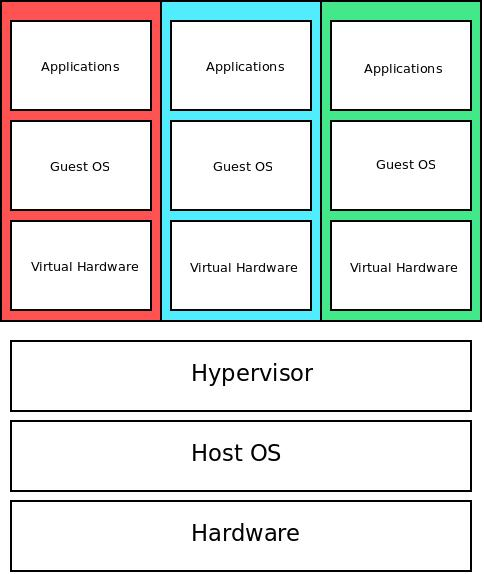
\includegraphics[width=10cm,height=10cm, keepaspectratio]{fullvirt.jpeg}%
  \caption{Full virtualisation architecture}
  \label{fig:full}
\end{figure}

The main advantage of full virtualisation is that it is easy to deploy and should not pose problems to an average user but the virtualisation overhead results in significantly reduced performance when compared to running directly on hardware. Popular examples of full virtualisation applications are Oracle's \textit{VirtualBox}\cite{VirtualBox} and \textit{VMware Workstation}\cite{WorkStation}. 

\subsubsection{Hardware-Layer virtualisation}

Hardware-Layer virtualisation is also a type of full virtualisation, but unlike Type 2 hypervisors, the so called \textit{Type 1 Hypervisors} (also \textit{native} and \textit{bare metal}) run directly on hardware. As seen on figure ~\ref{fig:hardware} there's no Host OS per se. Instead the Guest OSs access to hardware resources is controlled by the hypervisor.

\begin{figure}[ht!]
\centering
  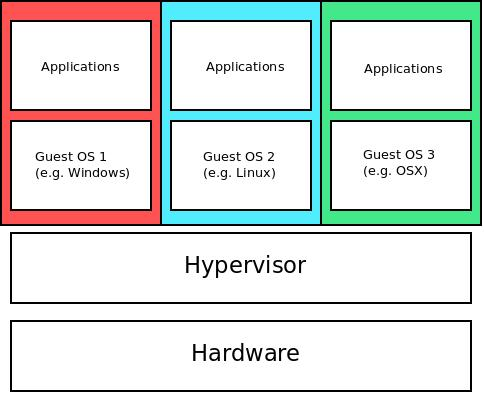
\includegraphics[width=10cm,height=10cm, keepaspectratio]{hwlayer.jpeg}%
  \caption{Hardware-Layer virtualisation architecture}
  \label{fig:hardware}
\end{figure}

Running directly on hardware, Hardware-Layer virtualisation techniques suffer less performance overhead than their OS-layer counterparts. On the other hand, Type 2 hypervisors being essentially applications themselves can be ran in parallel on the host OS whereas Type 1 hypervisors can not. For an average user, setting up a Type 1 hypervisor can be more difficult than Type 2. Commercial examples of Type 1 Hypervisors include Microsoft's \textit{Hyper-V}\cite{hyperv} and VMware's \textit{VSphere} \cite{vsphere}.

\subsubsection{Container-based virtualisation}

Instead of virtualising the underlying hardware, container-based virtualisation also known as OS-Layer virtualisation \cite{taxonomy} focuses on user space and allows running multiple operating systems in parallel as applications using the same kernel as the host operating system. A prime example of a popular container-based virtualisation platform is \textit{Docker} \cite{docker} which leverages on native Linux kernel features to virtualise and isolate OS instances. Figure ~\ref{fig:container} shows a container-based virtualisation architecture in which containerised environments are running operating systems on host OS's kernel. 

\begin{figure}[ht!]
\centering
  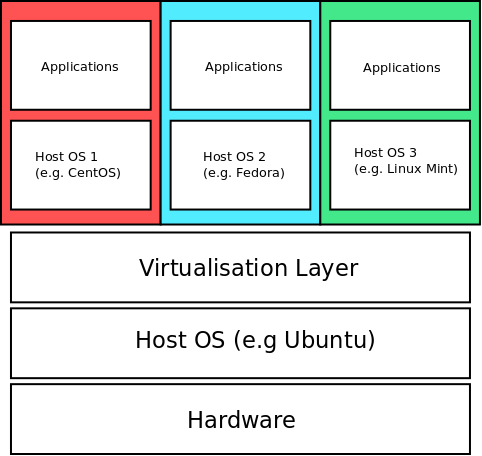
\includegraphics[width=10cm,height=10cm, keepaspectratio]{containers.png}%
  \caption{Container-based architecture}
  \label{fig:container}
\end{figure}

Container-based virtualisation does not need to emulate the hardware as containers communicate directly with the host kernel \cite{eder2016hypervisor} and are thus very fast to start. They also do not require all of the components a fully virtualised environment would need to run and therefore their resource fingerprint is minimal when compared to hypervisor-based virtualisation techniques. \linebreak
The obvious drawback of the technique is that the kernel of the virtualised OS has to be the same as that of Host OS e.g. In a situation depicted in figure ~\ref{fig:container} operating systems based on  Linux kernel could be ran on Ubuntu Host OS but OSs like Windows or OSX could not. On certain virtualisation platforms resource-intensive containers can also affect other containers detrimentally as the shared host OS's kernel is forced to spend its execution time on handling the instructions from the stressed container \cite{Xaviercontainer}.


\subsubsection{Paravirtualisation}

Paravirtualisation differs from full virtualisation by requiring the Guest OS to be modified in order to accomodate the virtual environment in which it is ran. Otherwise the architecture is similar to that of full virtualisation, but with thinner hypervisor allowing performance close to that of a non-virtualised environment. A well-known example of a paravirtualisation hypervisor is \textit{Xen}\cite{xen}.

\subsubsection{Unikernels}

Unikernels are a relatively recent take on virtualising services. Building on the notion that in cloud environments each VM usually specialises to provide only one service even if each VM contains a full-fledged general computer \cite{unikernels}. Unikernels are essentially minimal single-purpose library operating system (\textit{LibOS})\cite{libos} VMs with a single address space. They contain only the minimal set of services, implemented as libraries, built and sealed against modification to run the one application. Unlike the earlier LibOSes unikernels do not require a host OS to run but run directly on a VM hypervisor, such as Xen.

Some benefits of unikernels are obvious. Constructing VMs with minimal set of service libraries results in small images and resource footprints as well as fast boot times. Other benefits include reduced attack surface due to smaller codebase and sealing preventing any code not compiled during the creation of the VM from running. Single-address space improves context switching and eliminates the need for privilege transitions making system calls as efficient as function calls \cite{osv}. Running directly on the hypervisor instead of a host OS eliminates superfluous levels of hardware abstraction.

Optimisation and simplification are not without drawbacks. By definition, unikernels are not intended for general-purpose multi-user computing but for microservice cloud environments. Running multiple applications on a single VM is risky due single-address space does not offer any inherent resource isolation. As unikernels are sealed during compiling, it is not possible to do changes to them afterwards. User is instead required to compile and launch a completely new modified VM.

Popular examples of unikernels are \textit{MirageOS}\cite{mirage} and \textit{OSv}\cite{osv}.

\subsection{Experiment technologies}

This section discusses the technologies used and studied in the experiment in more detail. Virtualisation technologies are Docker, Xen, KVM and OSv and they are run on an OpenStack testbed.

\subsubsection{Docker}


\subsubsection{Xen}
\subsubsection{KVM}
\subsubsection{OSv}


\section{System Design and Implementation}

Current cloud management platforms make simplified assumptions about the hardware in the datacentre and its usage. Hardware is by default powerful rack or blade servers, they are virtualised and always on. Thus cloud management platforms on the market are suboptimal for certain use cases.

High Powered Computing (HPC) and Big Data applications require highly optimised and powerful hardware. In such applications, the overheads imposed by virtualisation are undesirable and for maximum efficiency the cluster should consist of the so-called bare-metal computing nodes. Furthermore other advantages of virtualisation such as multi-tenancy and scaling are not useful in bare-metal computing.

On the other end of the spectrum are very weak computers with limited computing power, memory, I/O throughput and storage. These machines can be a worthwhile addition to a cloud environment for running small low intensity tasks: They are significantly cheaper to traditional datacentre hardware costing some hundred euros per machine instead of thousands like a single rack server. They do not require much space to store, use less electricity and output less heat. Virtualisation may not be applicable for such machines either due to hardware not supporting virtualisation in the first place, or as the virtualisation overhead may consume large enough share of a machine's resources rendering it incapable to perform or at least severely restricting any other functionality besides virtualisation. With low end computers virtualisation benefits like multi-tenancy and running multiple operating systems in parallel may simply not be possible because of limited capabilities. Using these machines in a heterogeneous cluster requires treating them like a traditional bare-metal nodes, albeit not nearly as powerful.

In order to leverage on bare-metal nodes in a heterogeneous and possibly even in a hybrid cloud, the task schedulers require a view to the underlying infrastructure so that they can allocate tasks to nodes fitted to perform them. To extend the usage to befit hybrid clouds in addition to heterogeneous, the orchestrator has to be vendor agnostic too. This thesis presents prototype extensions to Cloudify's \cite{cloudify} client agents, which are used to communicate between the nodes and Cloudify Manager. Extensions are going to allow two things:

\begin{enumerate}
\item \textit{Allow the Manager to gain information about the nodes' hardware capabilities, a feature that is currently lacking from the project.}
\item \textit{Enable node discovery in the cluster.}
\end{enumerate}

Currently Cloudify does not allow adding nodes to the cluster while the cluster is operational. Especially with critical systems, failover in case of hardware failure is more difficult than with virtualised resources and the system administrators may not wish to bring the system offline to replace failed physical nodes. A discovery mechanism for new nodes in the cluster would ameliorate if not solve the problem, even if replacing faulty hardware is more often than not a manual task. Additionally discovery mechanism would allow \textit{Bring-your-own-host} kind of functionality.

 
\section{Technical Implementation}

% Do these need references?
Discovery Service is implemented with Python programming language and Flask Web framework. They were chosen because all of the components in Cloudify are also written in Python and Flask is used primarily for providing REST APIs. Even though Discovery Service does not provide any REST APIs, Flask is used for configuration management and source code organisation. Naturally, if need arises in the future to expand Discovery Service with a REST API, the development work is streamlined because of the framework.

In addition to Python program, Discovery Service relies on Redis \cite{Redis} as an in-memory key-value storage. Redis is a completely separate process in addition to Discovery Service. The preferred way of deploying Redis is in a docker container as it doesn't require installation or configuration save for exposing a correct port in the container and specifying Redis' address to Discovery Service. Redis could also be installed in the host system or even a remote system, though latter option has no practical purpose due to network latency as Redis achieves its high performance by storing values in the memory instead of disk.

\begin{figure}[ht!]
\centering
  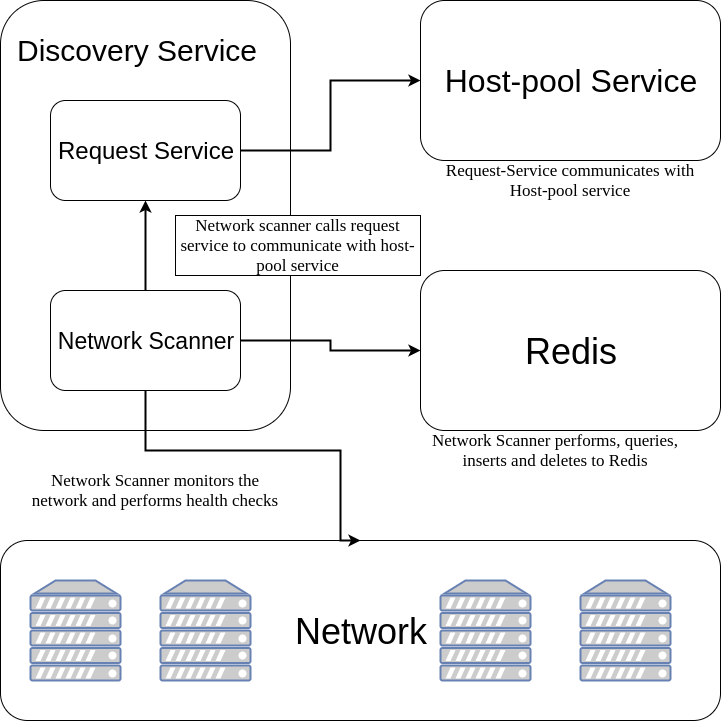
\includegraphics[width=12cm,height=12cm, keepaspectratio]{Discovery-service-communication.png}
  \caption{The communication relationships between Discovery Service and other components}
  \label{fig:communications}
\end{figure}

On the source code level, Discovery Service consists of two major components: The network scanner and request service. The network scanner is given a subnet as a parameter and it constantly sniffs the network detecting joining and already present devices and keeping track of them. Its other task is to periodically send health checks to known devices and if a health check fails enough times, it removes the given device from the logical host pool. Request service is responsible for sending HTTP requests to the Cloudify Host-pool service. It is called by the request service and it runs asynchronously. In addition to HTTP requests, it performs checks to ensure that the state of Discovery service's and Host-pool service's databases correlate.

The communication relationships between different components in the system are depicted in figure \ref{fig:communications}. The source code for Discovery Service as well as the documentation can be found at \url{https://bitbucket.org/Fleuri/discoveryserviceforcloudify/src/master/}

\subsection{Network Scanner}

The Network Scanner has two main functions, sniffer and pinger, and they run concurrently on two threads. Sniffer listens to ARP packets in the network and upon receiving one, stores the details of the sender device. Pinger function periodically sends ARP pings to previously discovered device and keeps track of their successes, eventually removing unresponsive devices from the logical host pool. In addition to two main functions there's a start-up function that initialises both local Redis storage and the Host-pool service's database. It pings all of the IP addresses in the given IP range and stores the found device details to databases.

\subsubsection{Sniffer}

Sniffer is started in its own thread during the start up sequence of the Discovery Service. It uses \textit{Scapy} library \cite{scapy} for Python. Sniffer function is given three arguments: 

\begin{enumerate}
\item \textbf{The network interface} which the Sniffer listens to for incoming packets.
\item \textbf{The callback function} which details further instructions to perform when a packet is caught.
\item \textbf{The filter} which restricts the type of packets caught.
\end{enumerate}

Only the interface can be set by the user of the Discovery Service. The callback function is the core application logic of the sniffer and the Discovery Service itself relies on sniffing ARP packets and therefore the filter is set accordingly.

When it comes to programming logic, the callback function is the most interesting part of the sniffer. Its purpose is to evaluate whether an ARP request comes from a new or know device and store details about them. When the function receives an ARP packet it first filters out packets that are not standard ARP requests. There are two such cases: ARP Probe \cite{rfc5227}, in which the source IP address or hardware address of the ARP request is \textit{0.0.0.0} or \textit{00:00:00:00:00:00} respectively, and gratuitous ARP in which the hardware address is \textit{ff:ff:ff:ff:ff:ff}. The user can also define a list of IP and hardware addresses which the Discovery Service should ignore i.e. devices on which Cloudify should not run workloads. Such devices include the host on which Cloudify manager runs and network devices such as routers.

Next the function checks whether the packet's origin is an already known host by querying Redis. If the host is not previously known or if it is a known device with a changed IP address, the function starts a new thread to add or patch the host to the Host-pool service. See section \ref{requestservice}.

Whether the packet's origin host is known or not, the next step in the function is to insert values extracted from the packet to Redis. The data structure Discovery service uses is simple, being a hash table with the devices' hardware address being a key and value being a dictionary object consisting of the given device's IP address and the number of failed ping attempts. See section \ref{pinger} for more details. If the packet's origin is a new host, its key and values are inserted to the data store with number of failed pings always being zero. If a device is already known, its hardware address is already stored to Redis and therefore its values are modified: in most cases only the failed ping count is reset to zero but there could be cases in which the device's IP address has changed and it is updated here accordingly. Algorithm \ref{fig:snifferalgo} details the structure of the function. Note that both adding a new host and patching an already known host is done in the same Request Service function. See section ~\ref{addtohostpool} for details.

\begin{algorithm}[H]
\label{fig:snifferalgo}
\begin{center}
\end{center}
\KwIn{Packet}
\If{Packet is an ARP packet}{
	\If{Packet is not an ARP Probe or Gratuitous ARP}{
	 	\If{Hardware address not found in Redis or IP address not found in Redis}{
	 	RequestService.Register\_a\_new\_host()\;
	 	}
		Redis.store(Packet.HardwareAddress: \{ip\_address: Packet.IPAddress, ping\_timeouts: 0\})\;
	}
}
\caption{Sniffer Callback Function}
\end{algorithm}

\subsubsection{Pinger} \label{pinger}

Pinger function is started in its own thread in the Network Scanner. Its responsibility is to keep track of the health of the nodes in the network. If Pinger discovers an unreachable node, it is removed from both Redis' and Host-pool service's storage.

Pinger periodically works through a list of known hosts in the network sending an ARP ping to each host. Upon receiving a response it resets the corresponding host's ping time-out counter to zero. If Pinger does not receive a response, it increments the given hosts' ping time-out by one. If after this operation the time-out crosses the given ping time-out threshold, the host is assumed to have disconnected from the network and is removed from the storage. After Pinger has pinged every host in the network, the process waits for a given ping interval after which it restarts the process.

The user gives inputs two parameters in a configuration file for Pinger to use: \textit{ping\_timeout\_threshold} and \textit{ping\_interval}. Ping\_timeout\_threshold specifies the maximum consecutive ping failures that can occur before a host is marked unreachable and removed from storage. Ping\_interval is the duration in seconds of which Pinger waits after each round of pinging the network. The more detailed presentation of the function is presented in the algorithm ~\ref{fig:pingeralgo}.

\begin{algorithm}[H]
\label{fig:pingeralgo}
\begin{center}
\end{center}

\While{True}{
	\ForEach{host in Redis}{
		timeouts = host.ping\_timeouts\;
		response = Ping(host)\;
	 	\If{response}{
	 		Redis.patch(host, \{ping\_timeouts: 0\})\;
	 	}
	 	\Else{
	 		timeouts++\;
	 		\If{timeouts >= ping\_timeout\_threshold}{
	 			RequestService.delete(host)\;
	 			Redis.delete(host)\;
		} \Else {
			Redis.patch(host, \{ping\_timeouts: timeouts\}\;		
		}		
	}
}
Sleep(ping\_interval)\;
}

\caption{Pinger Algorithm}

\end{algorithm}

\subsection{Request Service} \label{requestservice}

Request Service is responsible of communication between the Discovery Service and Host-pool Service. As seen on figure ~\ref{fig:communications}, it is called by Network Scanner and it makes requests to Host-pool Service. The REST API Host-pool Service provides is quite succinct but provides a typical CRUD interface for handling nodes in the network. The methods are as follows\footnote{\textit{Note: Paths are relative to Host-pool service base URL e.g. localhost:8081/hosts}} 

\begin{description}

\item[\textbf{[GET] /hosts}] \hfill \\
GET request to /hosts returns a JSON list of hosts and their details. Also accepts certain filters.

\item[\textbf{[POST] /hosts}] \hfill \\
POST request to /hosts with a valid JSON array will add one or more hosts to Host-Pool service's storage See listing ~\ref{lst:JSONformat} for the JSON schema definition. Returns Id’s of the new host or hosts.

\item[\textbf{[GET] /host/{id}}] \hfill \\
Returns details of a single host corresponding to the ID number.

\item[\textbf{[PATCH] /host/{id}}] \hfill \\
PATH request allows updating specified fields of a host with the given ID.

\item[\textbf{[DELETE] /host/{id}}] \hfill \\
Removes the host with given ID from Host-pool service's storage.

\item[\textbf{[POST] /host/allocate}] \hfill \\
This API call allocates a host to be used by the Cloudify Manager.

\item[\textbf{[DELETE] /host/{id}/deallocate}] \hfill \\
This returns a previously allocated host back to the host pool to be reallocated again.

\end{description}

Request Service interacts with all of the REST API endpoints except for allocation and deallocation endpoints which are interacted by Cloudify Manager's Host-pool plugin.

On source code level a typical Request Service function either makes an HTTP request to a certain endpoint, possibly with an ID corresponding to a host in the network, or constructs a JSON payload and sends that along with a POST request. Programmatic challenge in Request Service rises from the fact that the data model Host-pool service accepts is significantly more robust than that of the Discovery service, as can be seen on listing ~\ref{lst:JSONformat}. If Discovery Service's data model as seen on listing ~\ref{lst:discoformat} was a subset of Host-pool service's, handling data in Request Service would be trivial. However as Discovery Service's data model uses hardware addresses as unique identifiers whereas Host-Pool Service attaches a running number to each host. Hardware addresses are used as they are immutable in the cluster use-case and Discovery Service accounts for possibly changing IP addresses. However, Hardware addresses are by to Host-pool Service implicitly, as Discovery Service assigns each host's hardware address as a value for 'name' key. 

\begin{lstlisting}[language=json,firstnumber=1, caption={JSON schema accepted by the Host-pool Service for a single host}, captionpos=b, label=lst:JSONformat]
hosts: {
	id: Integer
	name: String
	os: String
	endpoint {
		ip : String
		protocol: String
		port: Integer	
	}
	credentials: {
		username: String
		password: String
		key: String
	}
	tags: Array
	allocated: Boolean
	alive: Boolean
}

NOTES:
- name is an arbitrary string, but Discovery Service assigns the host's hardware address as the value of name.
- os can be either 'linux' or 'windows'. Other values are invalid.
- endpoint.ip has to be a valid IP address range with CIDR notation. If a range is defined, Host-pool Service considers each unique IP address a single host.
- protocol can be either 'winrm-http', "'winrm-https' or 'ssh', but Host-pool service does not explicitly force this.
- Host-pool Service manages id, allocated and alive fields. For User, all other fields except credentials.password, credentials.key and tags are obligatory.
- In addition to 'hosts' key, Host-pool Service also accepts 'defaults' key. 'defaults' can contain the same keys as 'hosts'. If 'defaults' is provided, its values are appended to each host which has respective undefined values. id, allocated and alive cannot be provided as defaults.

\end{lstlisting}

\begin{lstlisting}[language=json,firstnumber=1, caption={Discovery Service data format for a single host}, captionpos=b, label=lst:discoformat]
hwaddress: {ip_address: "string", ping_timeouts:  "integer"}
\end{lstlisting}

\subsubsection{Id checking}

Due to differing identifiers, certain functions are implemented to keep the two data stores synchronized. A \verb|get_id()| -function retrieves a JSON object of hosts as depicted in algorithm ~\ref{fig:get_id}. Then it compares stored IP addresses for each host or until a match is found after which the ID is returned. If hardware address is passed as an argument, the function also compares it to \emph{name} -field's value, as Discovery Service names hosts in Host-pool Service after their hardware addresses. Hardware address check is used when Network Scanner finds an already known host with a changed IP address and calls Request Service to patch it to Host-pool Service. The ID itself is used for REST API calls that are directed at a single host.

\begin{algorithm}[H]
\label{fig:get_id}
\begin{center}
\end{center}
\KwIn{ip\_address}
\KwIn{hardware\_address = None}
\ForEach{host in RequestService.get\_hosts()}{
	\If{host.endpoint.ip is ip\_address or
		name is not None and 
		host.name is hardware\_address}{
	 		\Return{host.id}\;
	 	}
}
\Return{None}\;
\caption{get\_id -function compares stored IP addresses and optionally hardware addresses to find out the corresponding ID number in Host-pool Service.}
\end{algorithm}

\subsubsection{Adding a new host to Host-pool Service} \label{addtohostpool}

When Network Scanner detects a new host, it adds it to Redis key-value storage and starts a Request Service routine \verb|register_a_new_host| depicted in algorithm ~\ref{fig:addhost} in
a new thread to add the details also to Host-pool service. If a new IP address is detected but with an existing hardware address, the same routine is called. The \verb|register_a_new_host| function takes existing hosts into account and branches to patching function if need be. However, IP address changing for a host is a rare occasion and thus the function branching logic is done in Request Service for optimisation and maintaining source code readability.

\begin{algorithm}[H]
\label{fig:addhost}
\begin{center}
\end{center}
\KwIn{ip\_address}
\KwIn{hardware\_address = None}
{
stored\_id = get\_id(ip\_address, hardware\_address)
\If{stored\_id is None} {
	data = *formatted json object corresponding to host's details*\;
	response = *POST request to Host-pool Service with 'data' as payload.*\;
	\Return{response.json, message}
} \Else {
	\Return{RequestService.patch\_a\_host(stored\_id, ip\_address, hardware\_address)}
}
}

\caption{get\_id -function compares stored IP addresses and optionally hardware addresses to find out the corresponding Id number in Host-pool Service.}
\end{algorithm}

\subsubsection{Limitations and assumptions of the Discovery Service}

At its current prototypical state Discovery Service makes certain assumptions about the physical hosts in the cluster.
Namely hosts are assumed to have Linux as an operating system (Distribution can vary) and a default user name and a password, those being 'centos' and 'admin' respectively. In addition hosts are required to be running an SSH server which is a requirement enforced to Linux hosts by Cloudify itself. Discovery Service requires that the standard port 22 for SSH is open.
\section{Experiments} \label{experiments}

During development, the Discovery Service and Specification Retriever software were tested separately by mocking other elements in the Cloudify cluster. This section describes the experiments and their set-ups used to verify that different components integrate and work together flawlessly in a full environment built on real machines. The components in question are the aforementioned Discovery Service and Specification Retriever in addition to Host-Pool Service, Cloudify Manager, Host-Pool Plugin and the test workload, Cloudify Nodecellar Example\cite{Nodecellar}.

\subsection{Hardware set-up}
To verify that the Discovery Service and the Specification retriever function correctly in real environment and on real machines, I set up a test-bed depicted in figure ~\ref{fig:network-venn}.

 \begin{figure}[ht!]
\centering
  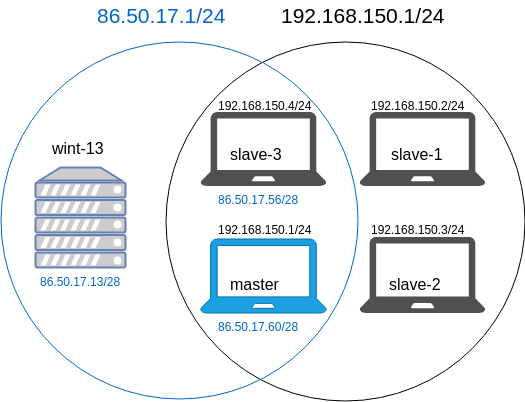
\includegraphics[width=\textwidth, keepaspectratio]{Network-venn.png}%
  \caption{The testbed hosts are located in a private network but master and slave-3 are also directly connected to network A.}
  \label{fig:network-venn}
\end{figure}

The test-bed consist of a Lenovo Thinkpad T420S 4173L7G laptop computer with  4-core Intel i5-2540M CPU and 8 GB of RAM acting as a master node in the Cloudify cluster. The three slave-machines are Lenovo Thinkpad Edge E145's with 2-core AMD E1-2500 APU CPUs and 4 GB of RAM. The master host has Centos 7 installed as the operating system to accommodate Cloudify's installation requirements. The three slave machines are running Ubuntu 16.04 as the OS of the slaves can be anything as long as they are Linux-based and the hosts themselves can be accessed via SSH.

\begin{figure}
\centering
  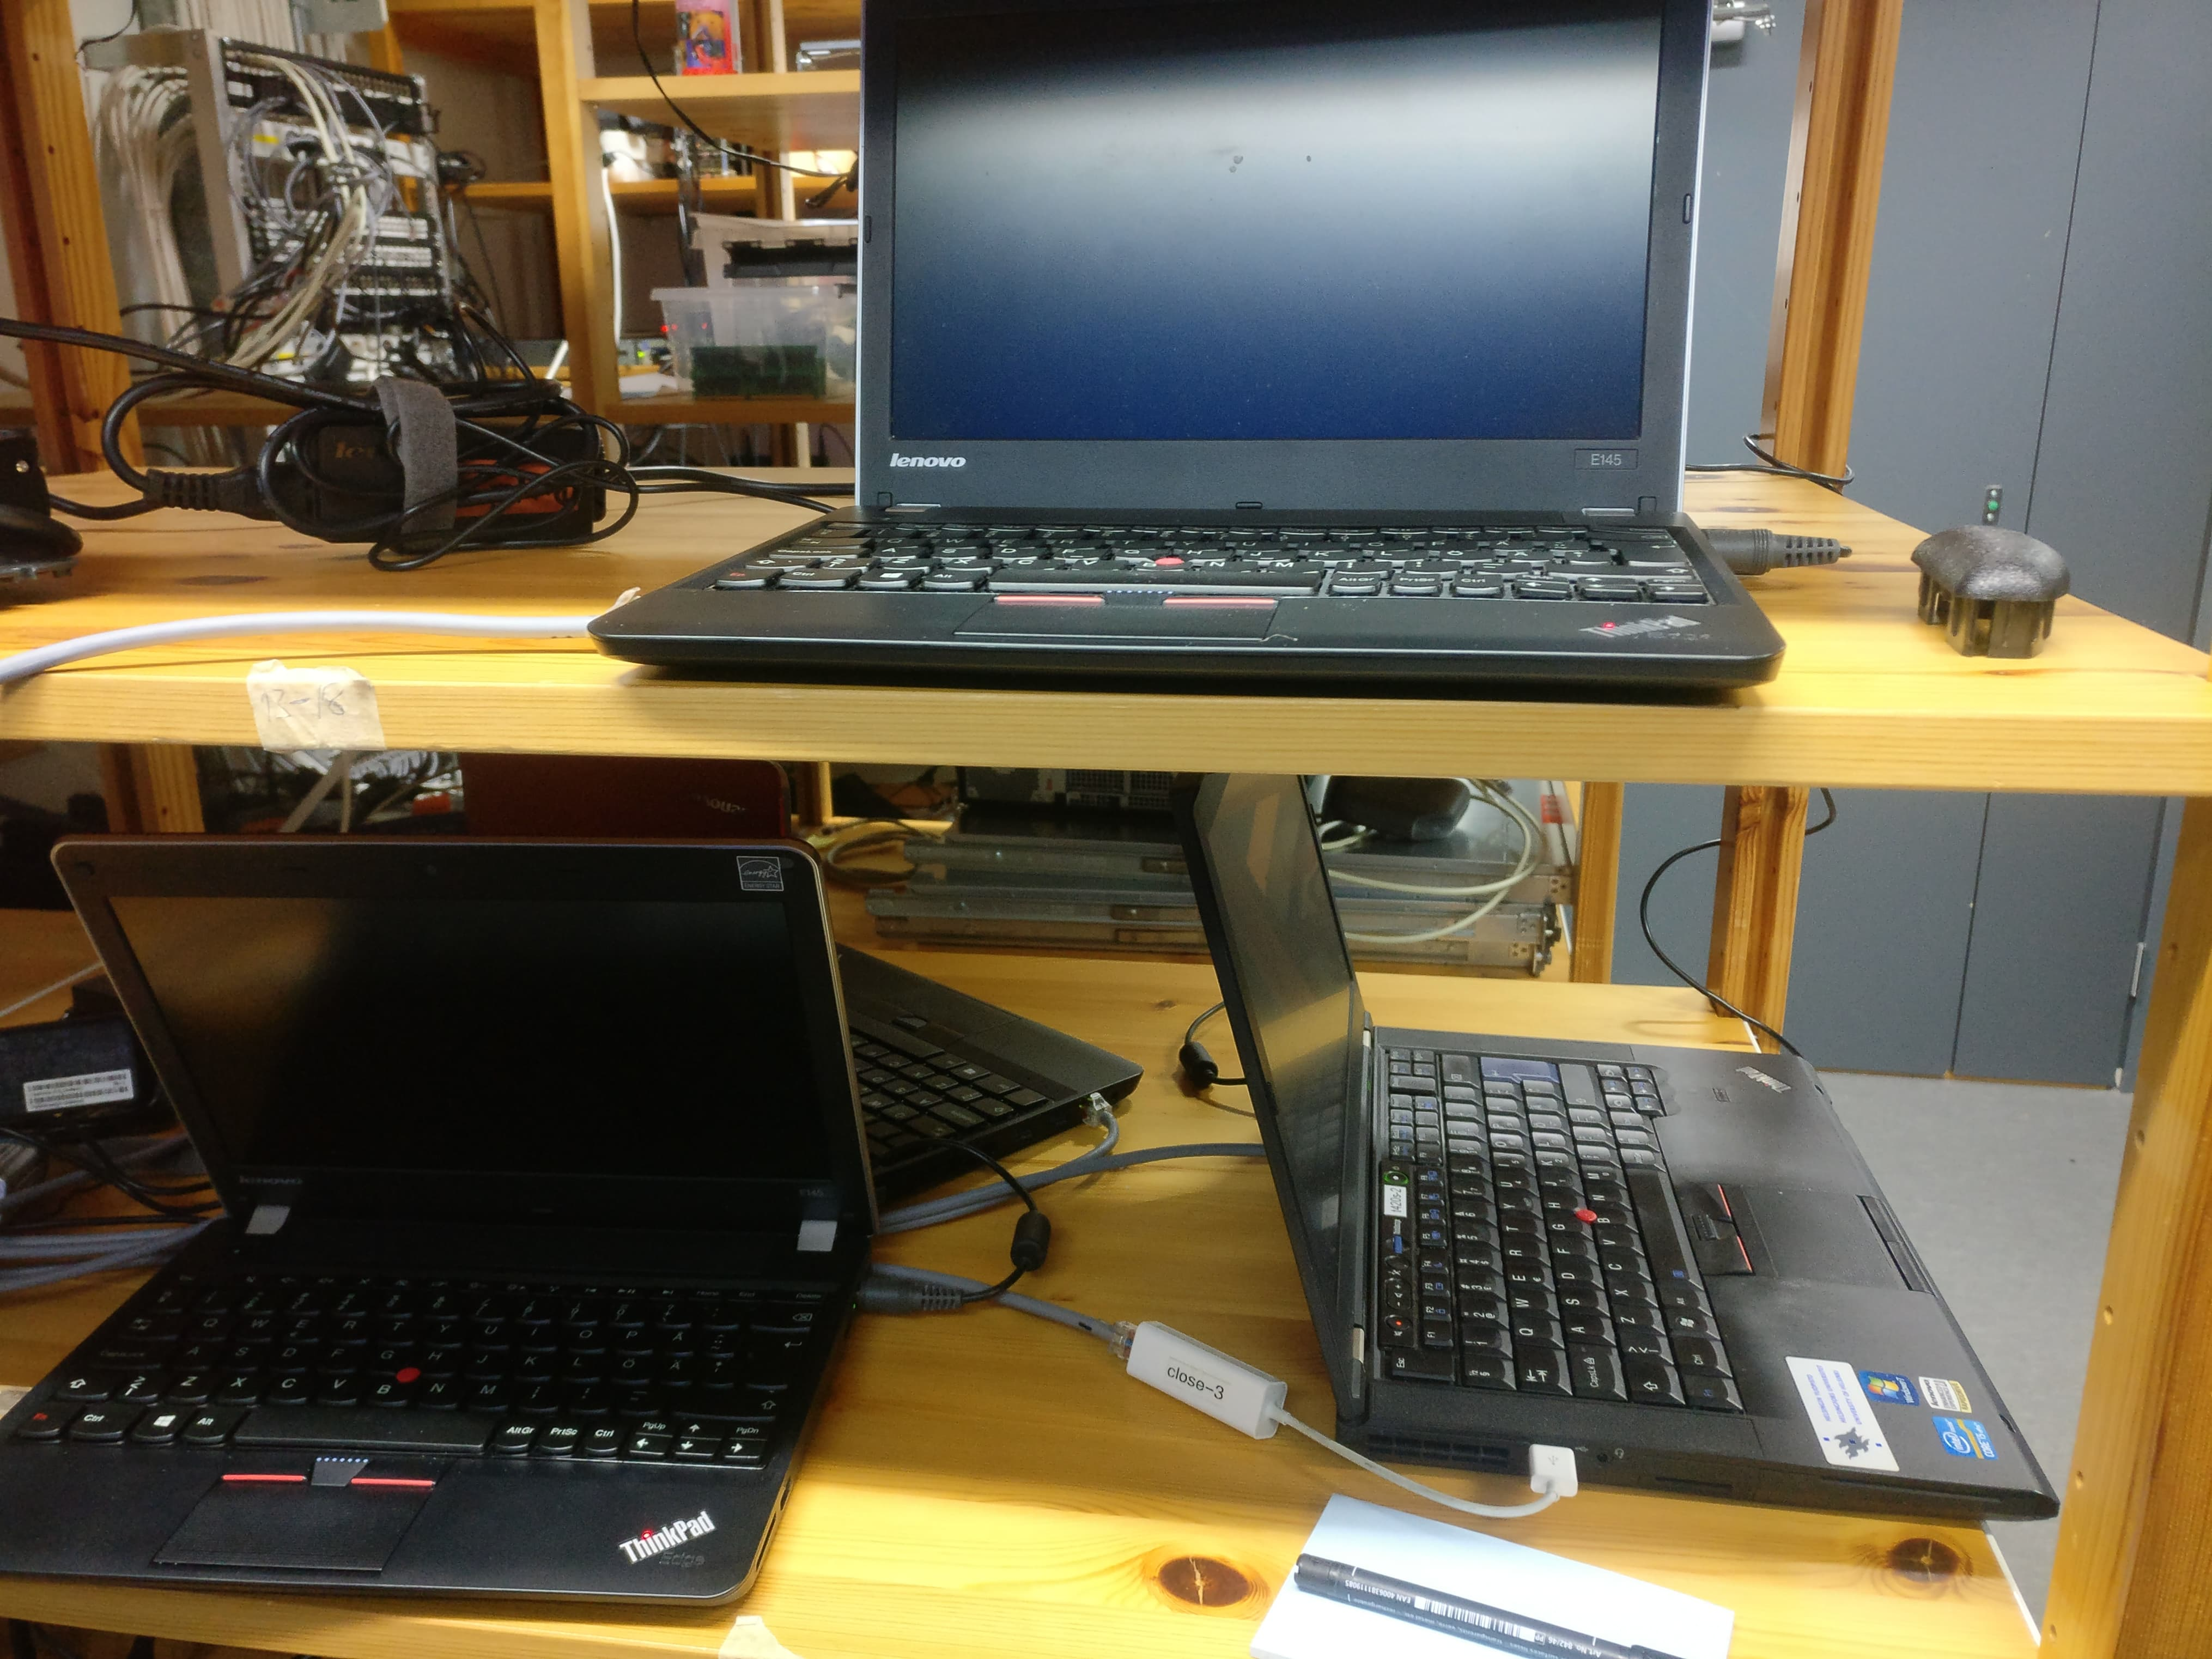
\includegraphics[width=12cm, height=12cm, keepaspectratio]{testbed.jpg}%
  \caption{The actual test-bed. Master node on lower shelf on the right, slaves in the upper and lower shelf}
  \label{fig:test-bed}
\end{figure}

As seen on figure ~\ref{fig:network-venn}, the test-bed set up has two different networks. The Master can be accessed remotely via a bastion host \textit{wint-13}. Wint-13 itself is not a part of the test-bed set up, but it is used to access the testbed remotely and allow internet access for and through the master host.

Master host has two network interfaces configured for each network it's a part of: The subnet A for outside access and B which is the subnet dedicated for the Cloudify cluster. Master also serves as a default gateway for all of the slaves. Figure ~\ref{fig:network-venn} shows how slave machines are part of the cluster subnet with static IP addresses. In addition slave-3 is also connected to the A subnet. This is to provide a way to drop the host off and connect it back the cluster network but still be able to access it remotely via external network. The physical network is wired with Ethernet cables connected to an HP 5412 zl V2 switch.

\subsection{Software environment set-up}

As mentioned previously, slave hosts do not have many software requirements besides running a Linux distribution as an operating system and having an SSH server installed and accepting connections on the standard port 22. In the test-bed they also have their IP addresses and network interfaces configured statically.

Master node is more intricate than slaves in addition to being more powerful. It has the similar requirements to slaves when it comes to SSH server, but additionally it also runs the programs listed on table ~\ref{table:software}. 

\begin{wraptable}{R}{\textwidth}
\begin{tabular}{|l|l|}
\hline
Software & Version \\
\hline
Cloudify Manager & 18.10.4~community \\
Host-pool Plugin within Cloudify Manager & 1.4 \\
Modified Host-pool Service & 1.2 \\
Discovery service & N/A \\
Docker & 1.13.1 \\
Redis running in a Docker container & 5.0.0 \\
\hline
\end{tabular}
\caption{List of software and their versions used in the experiment setup}
\vspace{10pt}
\label{table:software}
\end{wraptable}


\begin{wraptable}{R}{8cm}
\centering
\begin{tabular}{ | l | p{2cm} | }
\hline
Application & Port \\
\hline
\multicolumn{2}{|c|}{Cloudify ports} \\
\hline
Rest API and UI, HTTP & 80 \\
Rest API and UI, HTTPS & 443 \\
RabbitMQ & 5671 \\
Internal REST communication & 53333 \\
\hline
\multicolumn{2}{| c |}{Other ports} \\
\hline
SSH & 22 \\
Host-pool Service* & 5000 \\
Redis* & 6379 \\
\hline
\multicolumn{2}{| l |}{\textit{* Only internal access}} \\
\hline
\end{tabular}
%\begin{framed}
\caption{Required open ports on the master node. All ports are TCP}
%\end{framed}
\label{table:ports}
\end{wraptable}

In addition the master host has to expose a certain number of ports both internally and externally listed on table ~\ref{table:ports}.

Host-pool plugin runs as a Cloudify deployment managed by Cloudify manager. The modified Host-pool Service runs as a stand-alone Python program listening to port 5000. Even though Cloudify documentation recommends running Host-pool Service as a Cloudify Deployment on a separate host from Cloudify Manager, there are no drawbacks in this kind of local deployment either. 

The Discovery Service is also run as standalone program and it doesn't reserve any ports. However the key-value storage the Discovery Service uses, Redis, is run in a docker container using the official Redis docker image. It reserves the standard  Redis port 6379.

Finally, the server clocks on master host and slave-3 are synchronized with ntp against the ntp server located in network A, as synchronized time is needed for accurate measurement results in the experiments.
  

\subsection{Test cases}

To verify that different parts of the Discovery Service and Specification Retriever work in a real environment, I have come up with six test cases which test how different parts of the software integrate with a real system. First four of the test cases test Discovery Service's ability to monitor  the cluster network and deliver the current cluster status to the Host-pool Service. The fifth test verifies that the Specification Retriever script in the Modified Host-pool service collects the hardware data correctly and also showcases its expandability. Finally I am going to run an example workload in the cluster which uses the Discovery Service to manage its logical host-pool. This verifies that the system can be used as an addition in a real Cloudify cluster.

The time measurements from all of the applicable test cases are displayed in table ~\ref{table:measurements}. The table shows the fastest and slowest measured times, average and median times as well as standard deviation. All timed tests are run thirty times and the detailed report of the measurement results can be found in appendix ~\ref{testMeasurements}.

%\begin{landscape}
%\begin{table}
%\centering
%\begin{tabular}{ | l || l | l | l | l | l |}
%\hline 
%Test-case \& Time in seconds & Min & Max & Average & Median & Standard Deviation \\
%\hline \hline
%Start-up & 5.402588129 & 5.7881305218 & 5.5874319077 & 5.5766154528 & 0.0941250689 \\
%\hline
%Joining host & 0.083220005 & 0.2186000347 & 0.1519426159 & 0.1486098766 & 0.0406485995 \\
%\hline 
%Parting host & 40.3925600052 & 45.1373398304 & 42.5071433465 & 42.4735150337 & 1.3414346833 \\
%\hline
%Patching a host & 0.0368499756 & 0.0.0572497845 & 0.0481163859 & 0.0482549667 & 0.0044948944 \\ 
%\hline
%\end{tabular}
%\caption{Summary of measurements performed in the test cases}
%\label{table:measurements}
%\end{table}
%\end{landscape}

\begin{table}[t]
\centering
\begin{tabular}{  r | c | c | c | c | c }
{\bf Test-case} & {\bf Min} & {\bf Max} & {\bf Mean} & {\bf Median} & {\bf Std. dev.} \\
\hline
Start-up & 5.40 & 5.79 & 5.59 & 5.58 & 0.094 \\
Joining host & 0.083 & 0.22 & 0.15 & 0.15 & 0.04 \\
Parting host & 40.39 & 45.14 & 42.51 & 42.47 & 1.34 \\
Patching a host & 0.04 & 0.06 & 0.048 & 0.048 & 0.004 \\ 
\end{tabular}
\caption{Summary of measurement results.}
\label{table:measurements}
\end{table}

\subsubsection{Discovering hosts at start up}

As detailed in the section ~\ref{startup}, when Discovery Service is initialised it flushes all of the databases and performs an ARP scan for every IP address in the network. The time taking starts when the ARP scan itself starts and finishes after. The flushing of Host-pool Service's database and Redis are not included in the results. The scanning function imposes a two second wait time after the last packet is sent and the interval between each sent packet is 0,001 seconds.

\subsubsection*{Setting up the experiment}

 In this experiment I have modified the ARP scanning routine so that it measures the time it takes to scan through the 256 address network. The network itself contains three other hosts besides the master host which is ignored in the scan. This experiment does not require measurements from other servers and therefore no modifications or scripts are run on them. Additionally, the main function of Discovery Service is modified so that it runs the start-up routine thirty times and exits right after.

\subsubsection*{Results}

As seen in the table ~\ref{table:measurements}, scanning through a 256 address network takes approximately 5.6 seconds. This means that it takes approximately 22 milliseconds to send and receive an ARP request for a single host. The real value however varies as the requests may return out of sync and with varying intervals. Also the \verb|timeout| value which denotes the time spent waiting after the last request is set to relatively high value of two seconds.

Overall, all of the runs succeeded and there is no notable deviation in the distribution of times. In comparison to writing and providing host specification in JSON format, automatic scanning is significantly more efficient.

\subsubsection{Detecting a joining host} \label{joining_host}

One of the main features of the Discovery Service is the ability to detect machines joining the network in real time. In this test case Slave-3 is not initially connected to the cluster network. I have prepared a script which first returns a current time stamp on Slave-3 and then enables the network interface facing the cluster network. The sniffer algorithm on the Discovery Service is modified so that it too returns a time stamp upon detecting  a new host. As both hosts are synced against the same time server, the timestamps are comparable allowing me to measure a time it takes for Discovery Service to detect a host after it has joined the network.

\subsubsection*{Setting up the experiment}

This experiment required only a minor modification to Discovery Service's \verb|register_a_new_host| function which printed the timestamp to a file whenever Slave-3 was detected as a new host. Slave-3 was initially disconnected from the cluster network. On slave-3 a BASH script was run which first turns on the network interface to network B, sleeps fifteen seconds and sends an ARP request to the network while recording the timestamp. Then the script sleeps for a minute, turns off the interface and waits another minute until and starts over. The function was repeated thirty times.

\subsubsection*{Results}

As with the start-up scan, the time to detect a joining host is very regular and is more affected by the network speed rather than the implementation overhead. There were however outliers caused by the test implementation. As the network interface on Slave-3 was enabled there was a slight wait in the script execution so that the interface is ready before sending an ARP request. As the script was run multiple times, the ARP cache often did not have time to invalidate and thus no ARP request was automatically sent when the interface was ready, so manually sending the ARP request was necessary. In a real use case, such rapid enabling and disabling of the interface would be unlikely and the cache invalidation a non-issue. In few cases however, the cache was invalidated between a run and the ARP request was sent when interface was ready, causing the Discovery Service to catch the request before the time was recorded on Slave-3 resulting in a negative time in the final results. Those times have been disregarded in the table ~\ref{table:measurements} but are provided in the appendix ~\ref{testMeasurements}.

Overall most of time taken to detect a joining hosts consists of the interval between sending and receiving the ARP request.

\subsubsection{Detecting a departed host}

Similarly to detecting the joining host, detection of a departed host is another major feature of the Discovery Service. The testing procedure is also similar: Slave-3 has a script which drops the host from the network while producing a time stamp for the event. The departure detection in the Discovery Service is modified to return a time stamp when the detection of Slave-3 is detected. The detection is done in the pinger component described in section ~\ref{pinger}, in which a host is declared departed if it fails to reply to a set number of pings. The values for the ping interval and ping failures are five seconds for the interval and three failures. This relatively long interval is likely to cause a wide distribution of time results as the time between Slave-3 getting dropped from the network and the first ping could be five seconds. On the other hand this measurement is representable of a real usage scenario. \newline 

\subsubsection*{Setting up the experiment}

As in the previous experiment, only modification done to Discovery Service is producing a timestamp when Slave-3 is declared to have left the network. The script run on Slave-3 is also virtually identical to that of experiment ~\ref{joining_host} with the exception that the time stamp is recorded when the network interface is disabled. Slave-3 started disconnected from the cluster network in this case also.

\subsubsection*{Results}

Every execution of the pinging routine consists of two parts which make up the majority of the execution time. First the time out the ARP ping spends waiting for a reply is ten seconds and an interval between pings is five seconds. Depending on how fast a ping routine fires after Slave-3 disconnects, these parts take minimum of forty seconds and maximum of 45 five seconds.

Both extremums are presented in the experiment sampling and both average and median values are close to expected mathematical average. The computational overhead is negligible when compared to the ping interval and time out, but keeping that in mind, the average and median times could have been expected to be slightly over 42,5 seconds. 
Nevertheless, taking into account the expected five second variability of the beginning of execution, another data sample could result in slightly different times but similar standard deviation.

\subsubsection{Patching a host}

Procedure on this test case is similar to the previous two. A script modifies the IP address of Slave-3 from B.B.B.4 to B.B.B.5 and back, each modification producing a time stamp for in Slave-3 and each detected address change producing one on Master. Similarly to \textit{Detecting a joining host} experiment, an ARP request is sent manually as the ARP caches may not have time to be invalidated and thus changing the IP address may not trigger an ARP request automatically.

\subsubsection*{Setting up the experiment}

The experiment setup started similarly to previous two but instead of one function on Slave-3 to turn the network interface on and off, there needed to be two to alternate between .4 and .5 IP addresses using the network manager. Discovery Service's \verb|patch_a_host| function was modified to produce a timestamp whenever Slave-3's IP address was edited.

During the preliminary testing it became apparent that in some cases, as one IP address was unused for a longer time than for example in \textit{Detecting a parting host} experiment, ARP caches became invalidated more frequently. This meant, that changing an IP address triggered an automatic ARP call more frequently than first expected and capturing this behaviour required an another time stamp to be recorded in the script on Slave-3.

\subsubsection*{Results}

In the experiment, Slave-3 provided time stamp both when the interface was enabled and also when the ARP request was sent manually. The first time stamp prevented negative times in the results but the time itself didn't reflect a time it takes for the Discovery Service to detect and patch an IP change, but rather the time it takes for a the interface to be ready in this particular case. These values have been omitted from the results in table ~\ref{table:measurements} but they are included in the appendix ~\ref{testMeasurements}.

The tests succeeded on every execution. Patching seemed to be the most lightweight of the operations tested: The slowest execution time was circa 26 milliseconds faster than the fastest execution of the \textit{Detecting a joining host} experiment. This is because changing a single field in an existing data object is computationally significantly less demanding than creating a new data object with multiple fields.

Like the results from the previous experiments, \textit{Patching a host} results also indicate correct, fast and regular execution of the routine.

\subsubsection{Retrieving hardware data from the hosts}

This test case shows, that the modified Host-pool Service retrieves correct hardware data from the host. First the hardware data is listed manually on the target host. Next the start-up routine is run which adds all the hosts in the network to logical host pool. The modified Host-pool Service runs the hardware specification retrieval scripts when the hosts are added. Afterwards Host-pool Service can be queried to confirm that correct data was retrieved.

This test case also demonstrates how easily new commands can be added to the Specification Retriever.

\subsubsection*{Setting up the experiment}

This experiment did not require any additional modifications apart from additional commands described in the next section. However, correct values from Slave-3 were retrieved by hand as seen on figure ~\ref{fig:slave_3_specs} so that the values produced by the Specification Retriever could be verified. As values were static and slave hosts identical, the experiment was run only once.

\subsubsection*{Results}

 \begin{figure}[ht!]
\centering
  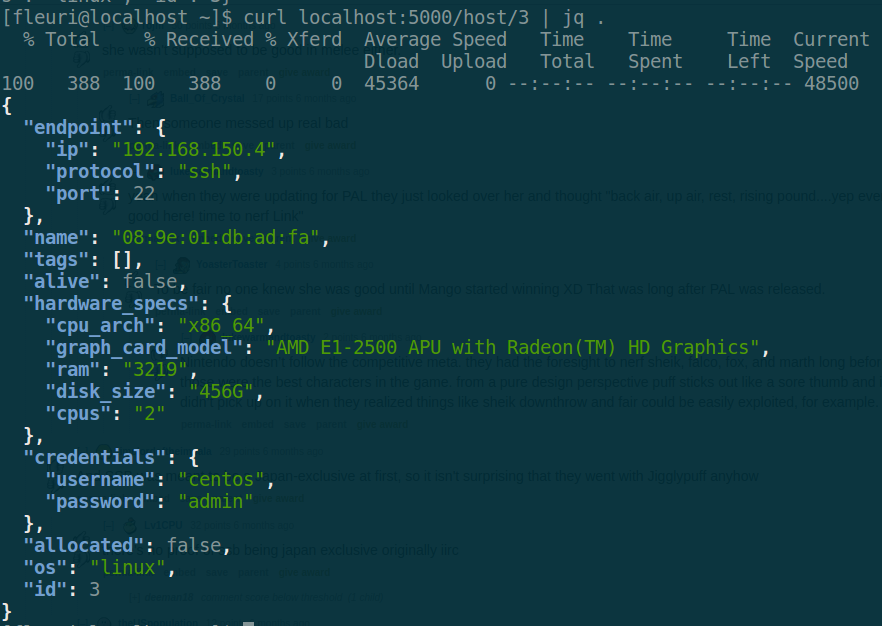
\includegraphics[width=\textwidth, keepaspectratio]{masterqueryscreenshot.png}%
  \caption{Host-pool service query returns a json with added new fields cpu\_arch and graph\_card\_model}
  \label{fig:master_query}
\end{figure}

 \begin{figure}[ht!]
\centering
  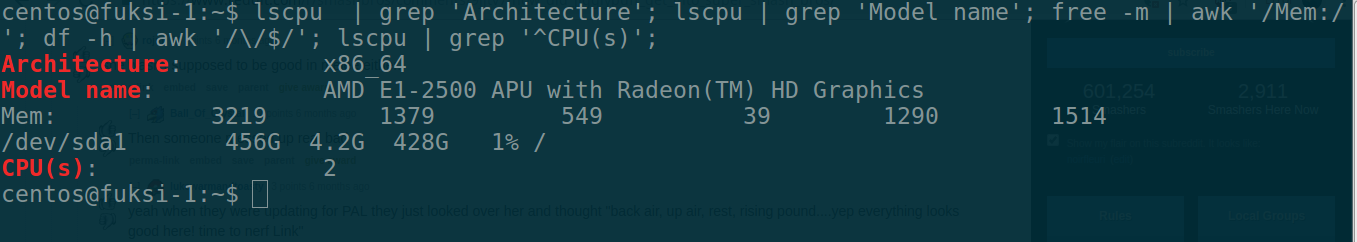
\includegraphics[width=\textwidth, keepaspectratio]{slave_3_specs_screenshot.png}%
  \caption{The results of individual commands run on Slave-3}
  \label{fig:slave_3_specs}
\end{figure}

Openstack's \textit{Ironic} -project\cite{ironic_troubleshoot} retrieves a modest amount of hardware data, namely the Number of CPUs, available RAM, available disk space and CPU architecture. CPU architecture retrieval was not included in the modified Host-pool Service specification detailed in section ~\ref{specification_retriever}, but to demonstrate specification retrievers capabilities and extendibility, I have added it as well as a command to retrieve the host's graphics card model to the list of commands executed on hosts. The commands are as follows:

\begin{itemize}
\item \verb= lscpu | awk '/Architecture/{ print \$2 }'= which retrieves the cpu architecture.
\item \verb=lscpu | awk '/Model name/' |= \linebreak \verb=sed -e 's/Model name://g' -e 's/^[ \t]*//g'= which retrieves the graphics card model while removing whitespace from the command result.
\end{itemize}

In the experiment the additional query commands were added to the modified Host-pool service. Discovery Service was ran normally and the Host-Pool Service REST endpoint was queried for Slave-3's data. Figure ~\ref{fig:master_query} is a screenshot of the query result and it shows the hardware data along with the added CPU architecture and graphics card model. Figure ~\ref{fig:slave_3_specs} is a screenshot showing the same data when queried directly on Slave-3 in remote terminal. The data in Host-pool service query is identical to that queried directly on Slave-3, verifying the correctness of the Hardware Specification retrieval operation. It also verifies, that the Hardware Specification retrieval operation can be easily extended with only minor additions to Host-pool Service.


\subsubsection{Running an example workload in the system}

 \begin{figure}[ht!]
\centering
  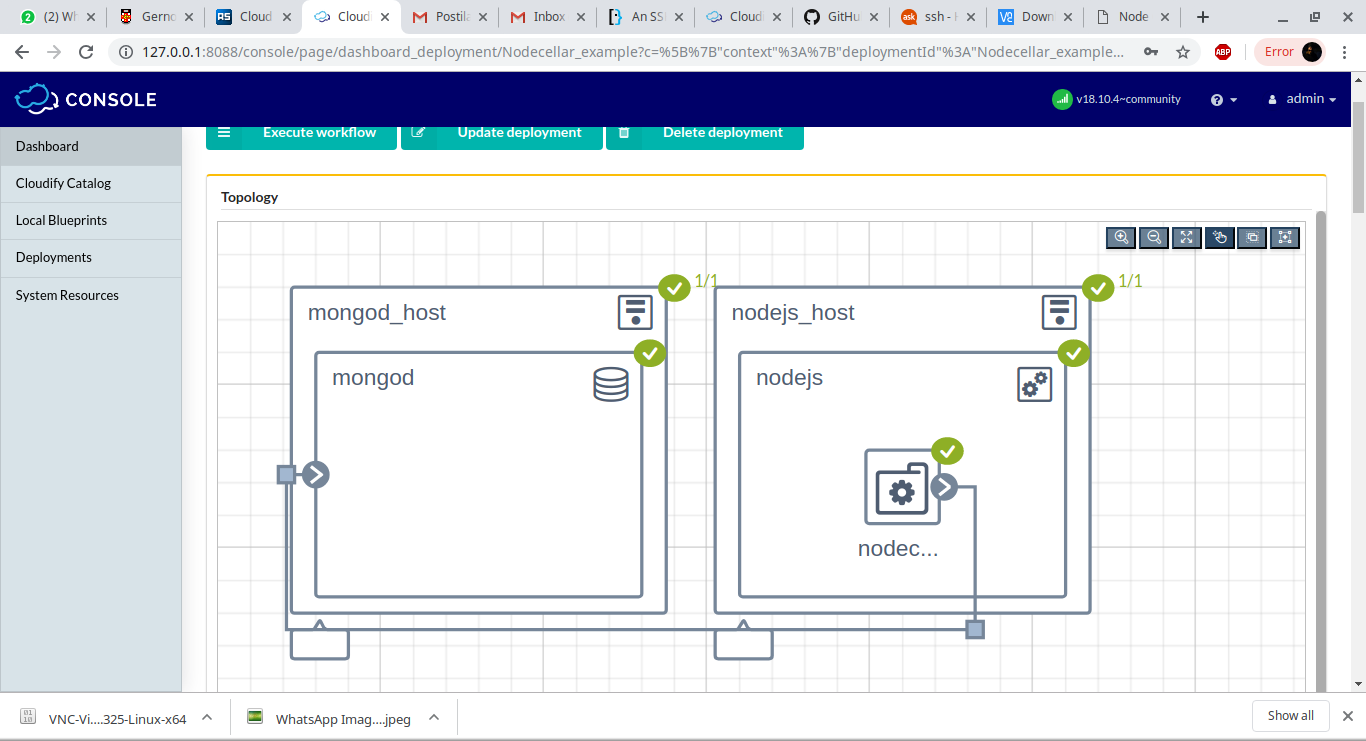
\includegraphics[width=\textwidth, keepaspectratio]{consoletopology.png}%
  \caption{Cloudify console shows the topology diagram of the Nodecellar deployment}
  \label{fig:console_topology}
\end{figure}

 \begin{figure}[ht!]
\centering
  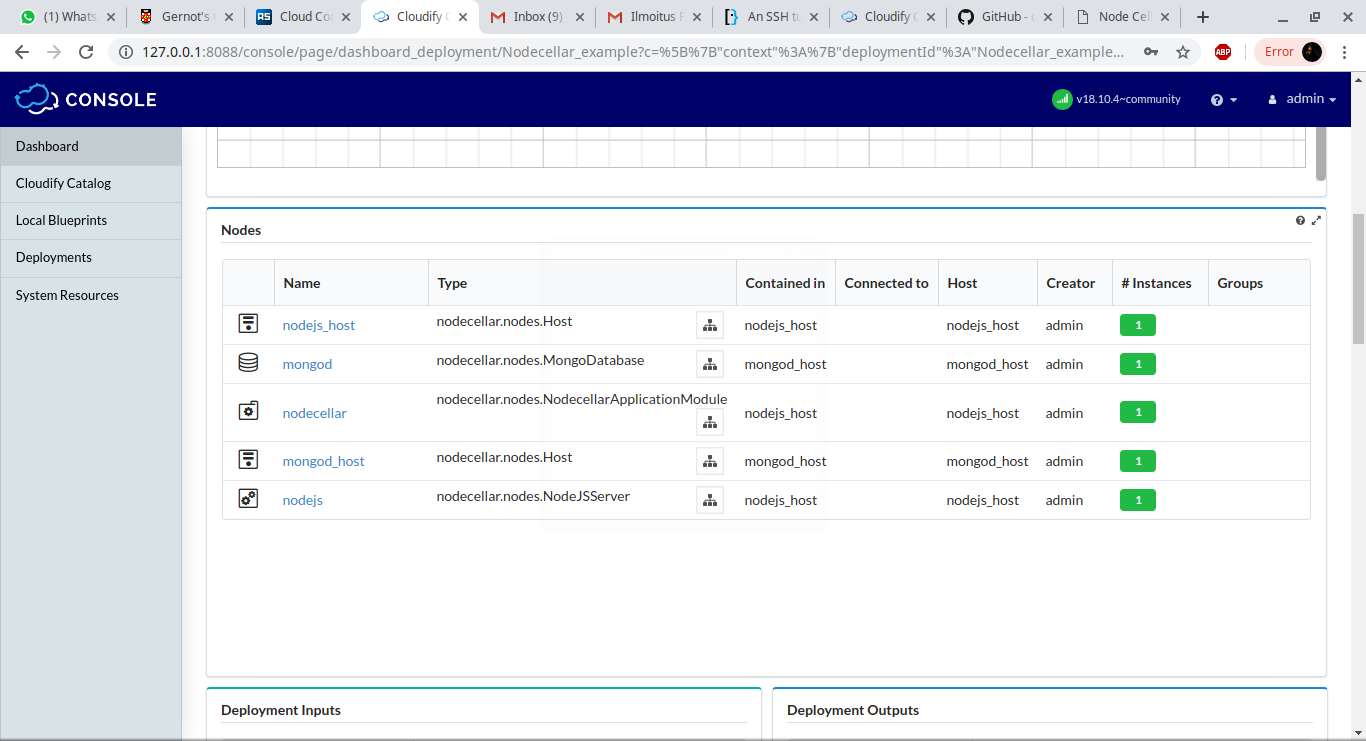
\includegraphics[width=\textwidth, keepaspectratio]{console_list.png}%
  \caption{Nodecellar deployment's parts listed in the Cloudify console}
  \label{fig:console_list}
\end{figure}

The final experiment shows, that Discovery Service works seamlessly when running a real workload in the Cloudify cluster. The workload in question is Cloudify's standard example workload Cloudify Nodecellar Example\cite{Nodecellar}. Nodecellar is a web application which simulates a wine inventory system. It is deployed on two separate hosts with the \textit{nodejs\_host} running a webserver and a Node.js based frontend application whereas the second \textit{mongod\_host} houses MongoDB. The figures ~\ref{fig:console_topology} and ~\ref{fig:console_list} are screenshots of the Cloudify console showing the different components of the Nodecellar deployment and the relations between them. The goal of this experiment is to have a functioning Nodecellar application running on two of the slave hosts which were discovered by the Discovery Service and allocated to Cloudify Manager by the Host-Pool Service.


\subsubsection*{Setting up the experiment}


 \begin{figure}[ht!]
\centering
  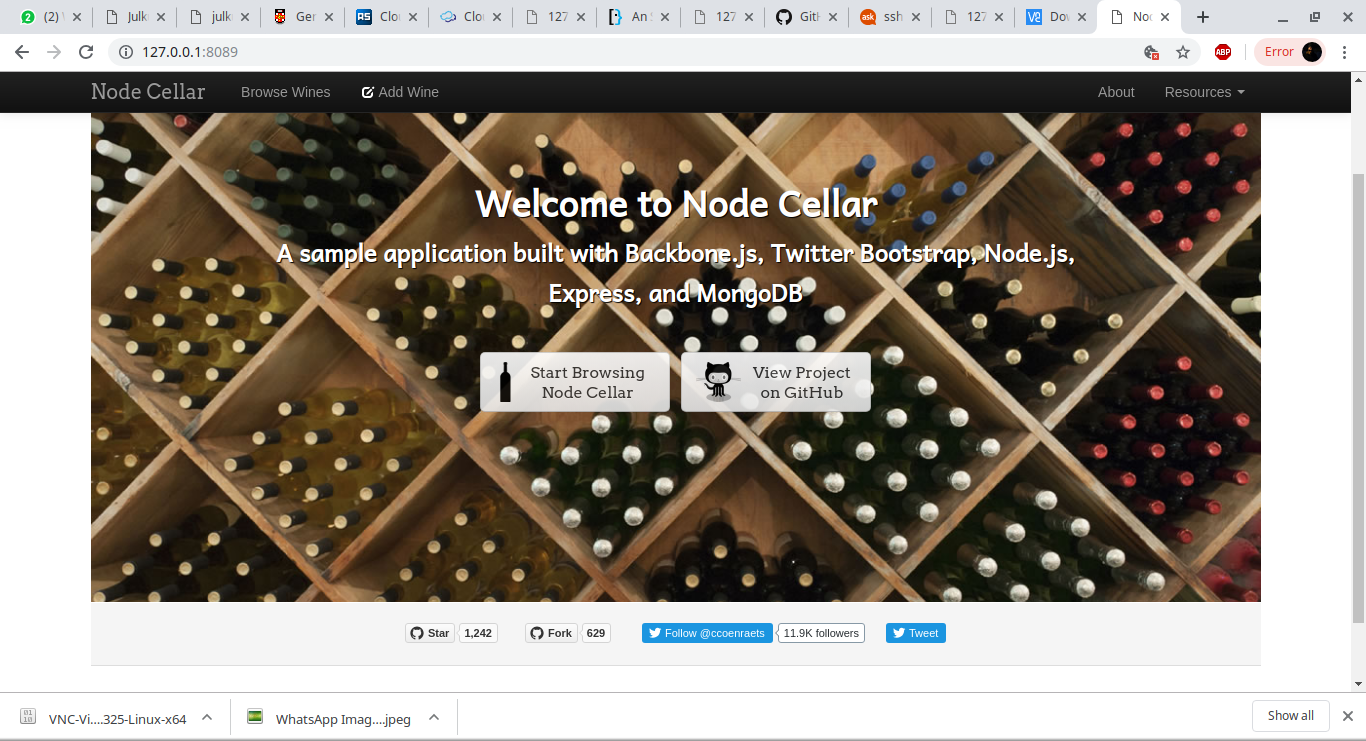
\includegraphics[width=\textwidth, keepaspectratio]{Nodecellarscreenshot.png}%
  \caption{Cloudify Nodecellar Example's landing page when deployed on the test bed cluster. The localhost IP address is due to port being forwarded to the \textit{node\_js} host.}
  \label{fig:nodecellar}
\end{figure}

 \begin{figure}[ht!]
\centering
  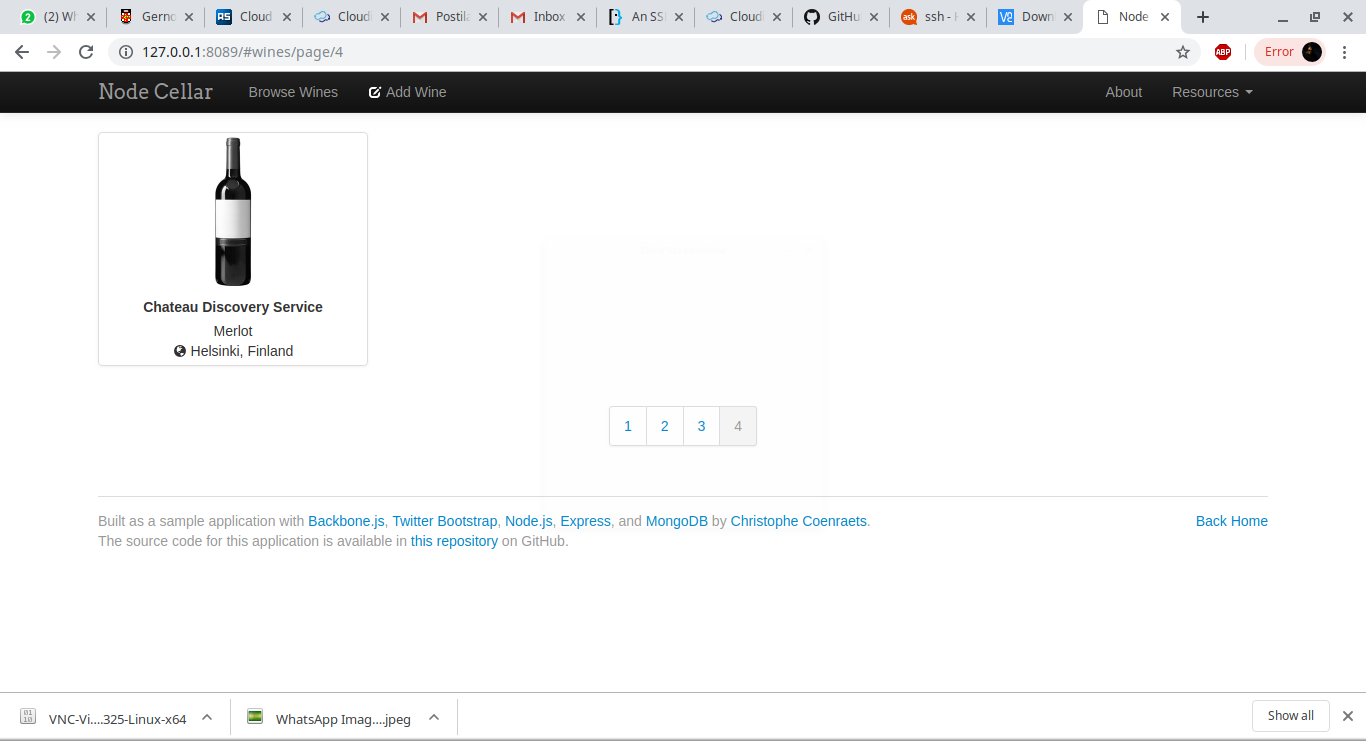
\includegraphics[width=\textwidth, keepaspectratio]{chateaudiscoveryservice.png}%
  \caption{Nodecellar allows the user to add their own wines to the list. This particular vintage is a real labour of love.}
  \label{fig:chateau}
\end{figure}

Prior to deploying Nodecellar, I had set up Host-pool Service, Discovery Service and Cloudify Manager. I had also forwarded the port of Cloudify Manager's web console so that I could access it remotely. On Cloudify, every component has to be defined as a Blueprint using TOSCA DSL. When blueprints are uploaded to Cloudify Manager, user can create Deployments of them which in turn create the actual resources.

Before Cloudify Manager could use Host-pool Service to allocate hosts for the deployment, the Host-pool Plugin was required to be installed. The latest version 1.5 was faulty so I downgraded to 1.4. This also meant that I had to manually change Nodecellar Example's blueprint's dependencies to use Host-pool Plugin version 1.4 instead of the default 1.5. After uploading the modified blueprints and creating deployments of them I ran the 'Install' workflow which requested the required hosts from Host-pool Service via Host-pool Plugin and after receiving them installed the required software on them.

\subsubsection*{Results}

As Host-pool Plugin allocates the requested available hosts in order, Slave-1 was designated as the \textit{nodejs\_host} and Slave-2 as \textit{mongod\_host}. To verify that the application is usable and served correctly I forwarded another port via wint-13 bastion host and Master host so that I could  view the web page on my local machine. Figure ~\ref{fig:nodecellar} shows a screenshot of the Nodecellar application. I could also add and remove wines to and from the system as seen on figure ~\ref{fig:chateau}. This validated that the MongoDB database on the second host as well as the connection between the hosts functioned correctly.

Overall it can be concluded that Discovery Service and the modified Host-pool Service function correctly in the experimental scope of this thesis.


\newpage
\section{Related work}
\section{Future Research}

Topics to be handled in this section

\begin{itemize}
\item {Robuster  error checking}
\item {Possibly unifying the data formats}
\item {Key handling}
\item {Robuster logging}
\end{itemize}
\section{Conclusions}




% --- References ---
%
% bibtex is used to generate the bibliography. The babplain style
% will generate numeric references (e.g. [1]) appropriate for theoretical
% computer science. If you need alphanumeric references (e.g [Tur90]), use
%
% \bibliographystyle{babalpha-lf}
%
% instead.

\bibliographystyle{babplain-lf}
\bibliography{references-en}


% --- Appendices ---

% uncomment the following

\newpage
\appendix
% 
\section{Test measurements} \label{testMeasurements}

\subsection{All start-up scan times}
% Please add the following required packages to your document preamble:
% \usepackage{longtable}
% Note: It may be necessary to compile the document several times to get a multi-page table to line up properly

\begin{longtable}{l|l|ll}
Run order & Time taken in seconds &  &  \\
\endfirsthead
%
\endhead
%
1 & 5.5212135315 & Average: & 5.5874319077 \\
2 & 5.6992228031 & Median: & 5.5766154528 \\
3 & 5.7459275723 & Fastest: & 5.402588129 \\
4 & 5.5203478336 & Slowest: & 5.7881305218 \\
5 & 5.402588129 & Standard Deviation:: & 0.0941250689 \\
6 & 5.5956482887 &  &  \\
7 & 5.5960564613 &  &  \\
8 & 5.6395816803 &  &  \\
9 & 5.5402934551 &  &  \\
10 & 5.5746655464 &  &  \\
11 & 5.5216667652 &  &  \\
12 & 5.5795629025 &  &  \\
13 & 5.7881305218 &  &  \\
14 & 5.6899979115 &  &  \\
15 & 5.5003581047 &  &  \\
16 & 5.6109347343 &  &  \\
17 & 5.5516016483 &  &  \\
18 & 5.6865930557 &  &  \\
19 & 5.7207539082 &  &  \\
20 & 5.6052863598 &  &  \\
21 & 5.5212519169 &  &  \\
22 & 5.7254798412 &  &  \\
23 & 5.6741354465 &  &  \\
24 & 5.5785653591 &  &  \\
25 & 5.5100474358 &  &  \\
26 & 5.5130033493 &  &  \\
27 & 5.4387583733 &  &  \\
28 & 5.5147643089 &  &  \\
29 & 5.5006010532 &  &  \\
30 & 5.555918932 &  & 
\end{longtable}

\begin{landscape}
\subsection{All host discovery times}
% Please add the following required packages to your document preamble:
% \usepackage{longtable}
% Note: It may be necessary to compile the document several times to get a multi-page table to line up properly

\begin{longtable}{l|l|l|l|ll}
Run order & Host joined network & Host found & Time taken in seconds &  &  \\
\endfirsthead
%
\endhead
%
1 & 1551985222.15239 & 1551985222.37099 & 0.2186000347 & \textbf{With negatives times} &  \\
2 & 1551985353.37076 & 1551985353.55532 & 0.1845600605 & Average: & -2.0597443342 \\
3 & 1551985484.60706 & 1551985484.69028 & 0.083220005 & Median: & 0.1445900202 \\
4 & 1551985615.83384 & 1551985615.97919 & 0.1453502178 & Fastest: & -9.4223599434 \\
5 & 1551985747.0425 & 1551985747.13216 & 0.0896599293 & Slowest: & 0.2186000347 \\
6 & 1551985878.28073 & 1551985868.89678 & -9.383949995 & Standard Deviation: & 4.0779027162 \\
7 & 1551986009.47946 & 1551986009.63293 & 0.1534700394 &  &  \\
8 & 1551986140.69389 & 1551986140.78502 & 0.0911300182 & \textbf{Without negatives times} &  \\
9 & 1551986271.93329 & 1551986272.12196 & 0.18866992 & Average: & 0.1519426159 \\
10 & 1551986403.17087 & 1551986393.87112 & -9.2997500896 & Median: & 0.1486098766 \\
11 & 1551986534.3891 & 1551986525.00583 & -9.3832700253 & Fastest: & 0.083220005 \\
12 & 1551986665.60635 & 1551986665.80476 & 0.1984100342 & Slowest: & 0.2186000347 \\
13 & 1551986796.82454 & 1551986796.97268 & 0.148140192 & Standard Deviation: & 0.0406485995 \\
14 & 1551986928.07304 & 1551986928.22165 & 0.1486098766 &  &  \\
15 & 1551987059.31184 & 1551987049.88948 & -9.4223599434 &  &  \\
16 & 1551987190.55872 & 1551987190.74462 & 0.1858999729 &  &  \\
17 & 1551987321.77601 & 1551987321.88523 & 0.1092200279 &  &  \\
18 & 1551987453.02166 & 1551987453.16549 & 0.1438298225 &  &  \\
19 & 1551987584.23665 & 1551987574.87545 & -9.3612000942 &  &  \\
20 & 1551987715.47122 & 1551987715.67965 & 0.2084300518 &  &  \\
21 & 1551987846.72406 & 1551987846.87137 & 0.1473100185 &  &  \\
22 & 1551987977.94288 & 1551987978.13356 & 0.190680027 &  &  \\
23 & 1551988109.16361 & 1551988099.90049 & -9.263119936 &  &  \\
24 & 1551988240.37602 & 1551988240.55236 & 0.1763401031 &  &  \\
25 & 1551988371.62402 & 1551988371.75052 & 0.1264998913 &  &  \\
26 & 1551988502.85096 & 1551988503.004 & 0.1530399323 &  &  \\
27 & 1551988634.07713 & 1551988624.90377 & -9.1733601093 &  &  \\
28 & 1551988765.32055 & 1551988765.51199 & 0.1914401054 &  &  \\
29 & 1551988896.54041 & 1551988896.63656 & 0.0961499214 &  &  \\
30 & 1551989027.77744 & 1551989027.89346 & 0.1160199642 &  & 
\end{longtable}
\end{landscape}

\begin{landscape}
\subsection{All host disconnection times}
  
% Please add the following required packages to your document preamble:
% \usepackage{longtable}
% Note: It may be necessary to compile the document several times to get a multi-page table to line up properly

\begin{longtable}{l|l|l|l|ll}
Run Order & Host Disconnected & Host Deregistered & Time taken in seconds &  &  \\
\endfirsthead
%
\endhead
%
1 & 1552122838.30771 & 1552122878.84452 & 40.5368101597 & Average: & 42.5071433465 \\
2 & 1552122969.52821 & 1552123010.39057 & 40.8623600006 & Median: & 42.4735150337 \\
3 & 1552123100.75055 & 1552123141.92967 & 41.1791200638 & Fastest: & 40.3925600052 \\
4 & 1552123232.00522 & 1552123273.43764 & 41.4324200153 & Slowest: & 45.1373398304 \\
5 & 1552123363.2187 & 1552123404.94401 & 41.7253100872 & Standard Deviation: & 1.3414346833 \\
6 & 1552123494.41722 & 1552123536.44338 & 42.0261600018 &  &  \\
7 & 1552123625.64917 & 1552123667.99715 & 42.3479800224 &  &  \\
8 & 1552123756.89979 & 1552123799.49884 & 42.599050045 &  &  \\
9 & 1552123888.12656 & 1552123930.99032 & 42.8637599945 &  &  \\
10 & 1552124019.33029 & 1552124062.49085 & 43.1605598927 &  &  \\
11 & 1552124150.55396 & 1552124193.94822 & 43.3942599297 &  &  \\
12 & 1552124281.7748 & 1552124325.49912 & 43.7243199348 &  &  \\
13 & 1552124413.01101 & 1552124457.04074 & 44.0297300816 &  &  \\
14 & 1552124544.22855 & 1552124588.53997 & 44.3114199638 &  &  \\
15 & 1552124675.45835 & 1552124720.04886 & 44.5905101299 &  &  \\
16 & 1552124806.6943 & 1552124851.50203 & 44.8077299595 &  &  \\
17 & 1552124937.91599 & 1552124983.05333 & 45.1373398304 &  &  \\
18 & 1552125069.14882 & 1552125109.54138 & 40.3925600052 &  &  \\
19 & 1552125200.36688 & 1552125241.03826 & 40.671380043 &  &  \\
20 & 1552125331.59595 & 1552125372.52238 & 40.9264302254 &  &  \\
21 & 1552125462.8262 & 1552125504.02815 & 41.2019500732 &  &  \\
22 & 1552125594.05397 & 1552125635.49851 & 41.4445397854 &  &  \\
23 & 1552125725.2785 & 1552125767.03705 & 41.7585499287 &  &  \\
24 & 1552125856.50981 & 1552125898.53611 & 42.0262999535 &  &  \\
25 & 1552125987.75468 & 1552126030.04648 & 42.2918000221 &  &  \\
26 & 1552126118.97288 & 1552126161.59271 & 42.6198301315 &  &  \\
27 & 1552126250.22228 & 1552126293.09072 & 42.8684399128 &  &  \\
28 & 1552126381.4452 & 1552126424.58656 & 43.1413600445 &  &  \\
29 & 1552126512.69665 & 1552126556.13836 & 43.4417099953 &  &  \\
30 & 1552126643.93728 & 1552126687.63789 & 43.7006101608 &  & 
\end{longtable}  
\end{landscape}

\begin{landscape}
\subsection{All host patching times}

% Please add the following required packages to your document preamble:
% \usepackage{longtable}
% Note: It may be necessary to compile the document several times to get a multi-page table to line up properly
\begin{longtable}{l|l|l|l|l|}
Run Order & Host patched & Arp sent after interface ready & Arp sent manually & Time taken in seconds  \\
\endfirsthead
%
\endhead
%
1 & 1554090361.33807 & 1554090351.28472 & 1554090361.29293 & 0.045140028 \\
2 & 1554090436.94233 & 1554090426.88258 & 1554090436.8893 & 0.0530297756 \\
3 & 1554090512.57653 & 1554090502.51601 & 1554090512.53004 & 0.046489954 \\
4 & 1554090588.14319 & 1554090578.07924 & 1554090588.09521 & 0.0479798317 \\
5 & 1554090663.74458 & 1554090653.68545 & 1554090663.69425 & 0.0503299236 \\
6 & 1554090734.77337 & 1554090729.30577 & 1554090739.31745 & 5.4676001072 \\
7 & 1554090814.9184 & 1554090804.86416 & 1554090814.87155 & 0.046849966 \\
8 & 1554090890.50323 & 1554090880.44033 & 1554090890.44953 & 0.0537002087 \\
9 & 1554090966.06846 & 1554090956.01977 & 1554090966.02604 & 0.0424199104 \\
10 & 1554091041.64256 & 1554091031.57167 & 1554091041.58865 & 0.053910017 \\
11 & 1554091117.22359 & 1554091107.16494 & 1554091117.178 & 0.0455899239 \\
12 & 1554091192.83752 & 1554091182.76329 & 1554091192.78027 & 0.0572497845 \\
13 & 1554091268.44217 & 1554091258.37663 & 1554091268.39109 & 0.0510799885 \\
14 & 1554091344.02731 & 1554091333.96437 & 1554091343.97667 & 0.0506398678 \\
15 & 1554091419.64087 & 1554091409.58761 & 1554091419.59896 & 0.0419101715 \\
16 & 1554091490.80174 & 1554091485.17243 & 1554091495.18706 & 5.6293098927 \\
17 & 1554091570.82652 & 1554091560.76264 & 1554091570.77351 & 0.0530099869 \\
18 & 1554091646.36245 & 1554091636.30388 & 1554091646.32124 & 0.0412099361 \\
19 & 1554091721.95576 & 1554091711.89861 & 1554091721.90741 & 0.0483500957 \\
20 & 1554091797.55627 & 1554091787.4974 & 1554091797.5077 & 0.0485699177 \\
21 & 1554091873.14775 & 1554091863.08645 & 1554091873.09959 & 0.0481598377 \\
22 & 1554091948.70667 & 1554091938.65154 & 1554091948.66079 & 0.0458800793 \\
23 & 1554092024.30841 & 1554092014.26166 & 1554092024.27156 & 0.0368499756 \\
24 & 1554092099.87953 & 1554092089.82066 & 1554092099.82925 & 0.0502798557 \\
25 & 1554092175.46025 & 1554092165.40143 & 1554092175.40846 & 0.051789999 \\
26 & 1554092251.07097 & 1554092241.01536 & 1554092251.02659 & 0.0443799496 \\
27 & 1554092326.70357 & 1554092316.65063 & 1554092326.65925 & 0.0443198681 \\
28 & 1554092402.28434 & 1554092392.2232 & 1554092402.23558 & 0.0487599373 \\
29 & 1554092477.83592 & 1554092467.77899 & 1554092477.78809 & 0.0478301048 \\
30 & 1554092553.37915 & 1554092543.3145 & 1554092553.3276 & 0.0515499115
\end{longtable}

% Please add the following required packages to your document preamble:
% \usepackage{longtable}
% Note: It may be necessary to compile the document several times to get a multi-page table to line up properly
\begin{longtable}{|ll|ll|}
\textbf{All value} &  & \textbf{No outliers} & \\
\endfirsthead
%
\endhead
\hline
%
Average: & 0.4148056269 & Average: & 0.0481163859 \\
Median: & 0.0484600067 & Median: & 0.0482549667  \\
Fastest: & 0.0368499756 & Fastest: & 0.0368499756  \\
Slowest: & 5.6293098927 & Slowest: & 0.0572497845 \\
Standard Deviation: & 1.3956489072 & Standard Deviation: & 0.0044948944
\end{longtable}

\end{landscape}
\end{document}